\documentclass[output=paper,colorlinks,citecolor=brown,nonflat]{langsci/langscibook}
\author{Anna Gudmundson	\affiliation{Stockholm University}}
\title{The mental lexicon of multilingual adult learners of Italian L3: A study of word association behavior and cross-lingual semantic priming}

\abstract{This study, a partial replication of the study conducted by \citet{FitzpatrickIzura2011} on bilingual speakers, investigates the structure and processing of the mental lexicon of multilingual speakers of first language (L1) Swedish, second language (L2) English and third language (L3) Italian in order of acquisition. By way of word association tasks in all three languages, the effect of language status (L1, L2, L3) and association category (i.e., the different kinds of word association responses) on reaction time (RT) and association distribution (i.e., proportion of associations in different association categories) is measured. Results show a significant effect of language status on association distribution and on RT. The present study also investigates the effect of long-term cross-lingual semantic priming and lexical mediation between L3 and L2 in a lexical decision task (LDT), i.e. if the activation of L3 conceptual information is mediated by the corresponding word form in the L2. The primes in this study are English words whose Italian translation equivalents were present in the prior L3 Italian word association task. The translation equivalents obtained shorter RTs compared to control words, which indicates that L2 English words were activated during the L3 Italian word association task. The kind of cross-lingual priming found in the multilinguals investigated in this study would imply that, besides the L1, also an L2 could mediate in lexical processing, and that the L1 does not have a privileged status in that respect.}
% \textbf{Keywords}: mental lexicon, crosslinguistic priming, word associations, proficiency, multilingualism, L1 Swedish, L2 English, L3 Italian

\shorttitlerunninghead{The mental lexicon of multilingual adult learners of Italian L3}
\begin{document}
\maketitle
\newpage

\section{Introduction}\label{sec:gudmundson:1}

Even though multilingualism has become a systematic research area over the last two decades (see \citealt{CenozEtAl2001, DeAngelis2007, GarciaMayo2012, Szubko-Sitarek2015}), especially within acquisition, sociolinguistics and teaching, according to \citet[1]{DeAngelis2007}, research on the cognitive and psycholinguistic aspects of multilingualism has been slow to appear. In addition to the so-called monolingual bias, \citeauthor{DeAngelis2007} discusses a bilingual bias which “overshadows the identification of a range of phenomena that only multilingual speakers can display” (\citeyear[13]{DeAngelis2007}), and which would be particularly pronounced in psycholinguistic research. According to \citet[10]{Szubko-Sitarek2015}, multilingual language users could be considered a new testing ground in psycholinguistics. The general objective of the present study is to contribute to filling the research gap discussed above. The study aims at shedding light on how the multilingual lexicon grows, and how lexical items from the different languages are interconnected. Particular attention is given to the role of the third language (L3), and to how L3 primes second language (L2) word activation. In this study, the terms first language (L1), L2 and L3 should be understood as referring to a chronological order of acquisition \citep{Hammarberg2014}.

The present study is a partial replication study of \citet{FitzpatrickIzura2011}, where word associations in bilingual participants of L1 Spanish and L2 English were explored. In their study, the types and the proportions of associative relations expressed in two word association tasks, first in the L1 and later in the L2, were analyzed to shed light on the structure, organization and development of the bilingual lexicon. An interesting part of the \citeauthor{FitzpatrickIzura2011} study was the adding of a lexical decision task in the L1 that followed the L2 association task. In the lexical decision task, some of the items were translation equivalents to stimuli words from the previous L2 association task. Results revealed a long-term cross-language semantic priming effect for those items, and that finding was interpreted in favor of the revised hierarchical model (RHM) (\citealt{KrollStewart1994}). The effect was explained by a lexical mediation effect between L2 and L1 that had taken place during the L2 word association task. The activation of the meaning of the L2 stimulus word had been mediated, according to \citeauthor{FitzpatrickIzura2011}, by first activating the corresponding L1 word form. That activation left a trace and served as a prime in the following L1 lexical decision task. The present study follows the same design as the one implemented by \citet{FitzpatrickIzura2011}, but contrary to their study, it focuses on multilingual speakers of a new language combination, L1 Swedish, L2 English and L3 Italian. Word associations in all three languages are analyzed, and a lexical decision task is performed, but instead of investigating priming between L2 and L1, as in the study by Fitzpatrick \& Izura, it investigates whether such a long-term priming effect can occur between the L3 Italian and the L2 English, i.e. if also an L2 can mediate access to conceptual information and what implications would follow as concerns the basic functioning of the RHM.

The structure of the introductory part of this paper is as follows: In \sectref{sec:gudmundson:1.1} and \ref{sec:gudmundson:1.2}, a presentation of the mental lexicon, both in L2 and in L3 is given. In \sectref{sec:gudmundson:1.3}, long-term cross-language semantic priming is discussed, while \sectref{sec:gudmundson:1.4} gives an outline of the functioning of word association studies. Finally, in \sectref{sec:gudmundson:1.5}, the different types of word relations identified by \citet{FitzpatrickIzura2011} are presented.

\subsection{The mental lexicon}\label{sec:gudmundson:1.1}

By mental lexicon, we mean a language user’s knowledge about words, i.e. a mental representation of all the words known by a user, their meaning, their form and their internal relations \citep{Aitchison2012}. The mental lexicon is often described as a network of connections between words, or features of words \citep{Aitchison2012}. These connections could be based on formal or semantic similarities. The semantic similarities create semantic fields composed of words with related meanings. Learning the meaning of new words involves creating connections to other words within the network, which is then reconstructed. The mental lexicon, from that point of view, is not static, but is continually changing in a dynamic way when new words are added or when our knowledge of a word is deepened. \citet[209--210]{Aitchison2012} uses the metaphor of a bookshelf that needs constant rearrangement when new books are added, based on their content and form. The depth-of-word-knowledge, i.e. a word’s different sense relations, is linked to lexical network building in the sense that knowledge of single words increases when new words are added and when we adapt and differentiate existing lexical links. Knowledge about words and their meanings is in such defined as a word’s relation to other words and it increases with breath-of-knowledge, i.e. vocabulary size (\citealt[222]{HaastrupHenriksen2000}; \citealt{Nation2001, Read2004}).

Another relevant concept when discussing the mental lexicon of an L2 learner is the speed with which a lexical item is accessed or processed. \citeauthor{Pellicer-Sánchez2015} states that “[i]t is uncontroversial that the ability to process language quickly is a component of more advanced language proficiency” (\citeyear[127]{Pellicer-Sánchez2015}). Being able to access and retrieve lexical information in a fast and efficient way is important for a learner’s capacity to speak fluently. Speed of lexical access is also referred to as automaticity \citep{Schmitt2010} in the sense that it measures procedural, implicit and unconscious knowledge. \citet[371]{SegalowitzHulstijn2005} argue that, generally, automaticity implies the absence of intentional control when a cognitive activity is executed. Learners go through an automatization process that is related to proficiency – with increasing proficiency, processing time diminishes and the number of errors decreases (\citealt{DeKeyser2007}). Thus, lexical access should be faster in more proficient language users compared to less proficient language users. Measuring reaction times in different kinds of language processing is a common way to establish automaticity (see \citealt{SegalowitzHulstijn2005} for an overview). \citet{SegalowitzSegalowitz1993} and \citet{SegalowitzHulstijn2005} state that, even though speed of lexical access is an important factor in determining automaticity, equating it to automaticity is problematic. They explain that increased speed could be the consequence of two different mechanisms, the first being general quantitative speed-up, and the second being a qualitative change in the processing mechanism itself. Only the second one could be identified as a change in automaticity. \citet{SegalowitzSegalowitz1993} suggest that automaticity be calculated as the standard deviation divided by mean reaction time. However, although this definition might be more linked to our understanding of the concept of automaticity, the method has been questioned \citep{HulstijnEtAl2009}. To avoid problems related to the concept of automaticity, in this study, increased reaction times will simply be interpreted as increased fluency, no matter what the determining mechanisms are.

{\sloppy The internal structure of the lexical item itself is often described as composed of two different levels of representation \citep{Levelt1989}. One level encodes semantic information or meaning and the other encodes its phonological form. In the present study the terms \textit{semantic representation}, \textit{conceptual representation} and \textit{meaning representation} will be used synonymously. Most research on the\linebreak monolingual mental lexicon is concerned with how the level of semantics and the level of meaning interact (\citealt{DellOSeaghdha1991, DellOSeaghdha1992, LeveltEtAl1991Picture, LeveltEtAl1991Reply, Levelt1992}), while research on the bilingual lexicon focuses on two other fundamental questions. The first question is whether lexical representations from different languages are stored together (the integrated view) or separately (the separate view), and the second question is whether lexical access is language selective or non-selective. On seeing the English word \textit{pencil}, is information of words from all languages known by the user activated, or only from those belonging to English (\citealt{Weinreich1953, SánchezCasasEtAl1992, Poulisse1997, DijkstraVanHeuven1998, DijkstraVanHeuven2002, VanHeuvenEtAl1998, VanHeuvenEtAl2011, Dijkstra2003, Dijkstra2005, LemhöferDijkstra2004, LemhöferEtAl2004, Costa2005,  KrollDeGroot2005, LaHeij2005, DijkstraEtAl2010, KrollEtAl2010, DeAngelisEtAl2015})?}

Many models of bilingual mental representations are inspired by the early work of \citet{Weinreich1953}, who proposed three different approaches to bilingual representations. The compound approach predicts different lexical stores but a shared conceptual store, while the coordinate approach predicts separate conceptual and lexical stores. Finally, the subordinate approach predicts a store for L1 conceptual representations only, while L2 lexical items are connected to these representations indirectly via the L1 translation equivalent. Evidence was found for the compound approach \citep{PotterEtAl1984}, but \citet{KrollCurley1988} found a difference between learners at different proficiency levels; less proficient learners performed according to the subordinate approach (also known as the word association hypothesis), and the more advanced learners according to the compound approach (also known as the concept mediation hypothesis). \citeauthor{KrollCurley1988} therefore suggested a switch from lexical to conceptual mediation as learners became more proficient. That idea was later developed into the revised hierarchical model (RHM) (\citealt{KrollStewart1994, KrollEtAl2010}), see \figref{fig:gudmundson:1} below, which combines the subordinate and the compound approaches into a single one.

\begin{figure}
    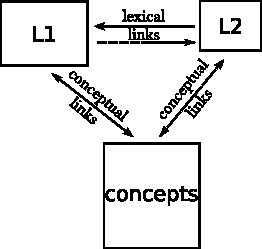
\includegraphics[height=.3\textheight]{figures/Gudmundson-fig1mod.pdf}
    \caption{Illustration of the RHM (adapted from \citealt{KrollStewart1994}).\label{fig:gudmundson:1}}
\end{figure}

The black solid arrows represent strong and well-developed links between word form representations and concepts, while the dashed arrows represent less well-developed links. The strength of the links varies as a function of proficiency. The model states that for less proficient L2 learners, access to meaning is mediated by L1 word forms as represented by the solid arrows, and it is only when higher proficiency levels are reached that direct links between L2 word forms and meanings are developed. The RHM also accounts for the longer translation latencies in backward translation (from L1 to L2) compared to forward translation (from L2 to L1), observed in many studies, by proposing asymmetrical links between the two languages. In backward translation, the process is mediated by semantic access, i.e. the L1 word form activates the conceptual information by way of the black solid slanted line, and in a second step the corresponding L2 word form. In forward translation, on the other hand, no semantic access is necessary due to direct lexical links between L2 word forms and L1 word forms. This is represented in the figure by the black solid horizontal line. Backward translation thus requires an additional processing step. Even though, according to the RHM, faster translation time in the forward condition is explained by the fact that it does not involve semantic access, semantic priming effects have been observed in other studies (\citealt{DuyckBrysbaert2002, SchoonbaertEtAl2009}). The absence of such an effect in earlier studies has been explained by a combination of two opposing effects that counterbalance each other: a facilitation effect and an interference effect (\citealt{WuJuffs2019}). The RHM has been used to analyze and describe the representation and processing of the bilingual mental lexicon. However, as pointed out by \citet[236]{GoralEtAl2006}, “[t]he model does not specify a priori whether words from additional non-native languages, learned after L2, are connected in the lexicon via the L1 words or L2 words”, and as noted by \citet{Singleton2003} and \citet{DeAngelis2007}, there is nothing in Weinreich’s work that indicates what would be the result when adding a third language to the already existing ones, something that will be investigated in the present study.

Models of bilingual word processing include, among others, the Inhibitory control model (\citealt{Green1986, Green1998}), the language mode framework (\citealt{Grosjean1997, Grosjean2001}) and the bilingual interactive activation model (BIA+). The BIA+ was elaborated by \citet{DijkstraVanHeuven2002} and presupposes an integrated lexicon, integrated semantic representations, and non-selective access. According to this model, the presentation of a word in one language activates, in parallel, lexical representations in both languages and, in a second phase, the corresponding semantic representations. The activation resonates within the network and the candidate reaching the highest level of activation is identified. The model does not predict any processing differences between the languages known by a user. There is a difference between the concept of co-activation as described above and that of linguistic mediation proposed by \citet{KrollStewart1994} and \citet{FitzpatrickIzura2011}. Mediation by an L1 is said to occur as a necessary step in L2 semantic processing at beginner level, but it ceases to occur in more advanced learners. Co-activation on the other hand, is something that happens regardless of proficiency levels, and it is not a phenomenon that, in the first place, helps learners to access lexical meanings in later learned languages.

The BIA+ is built on results from studies of the so-called cognate effect and the interlingual orthographic neighborhood effect, identified in lexical decision tasks (\citealt{SánchezCasasEtAl1992, LemhöferDijkstra2004, Dijkstra2005}). The cognate effect derives from the discovery that cognate words (i.e., words that have similar forms between languages and share the same meaning) are identified faster compared to non-cognates (\citealt{LemhöferDijkstra2004}). The interlingual orthographic neighborhood effect, on the other hand, derives from results showing that lexical items that are orthographically similar to many words in another language are identified more slowly compared to words that do not have the same number of orthographic neighbors, due to increased co-activation and competition (\citealt{GraingerDijkstra1992, VanHeuvenEtAl1998}).

\subsection{Studies of the L3 mental lexicon}\label{sec:gudmundson:1.2}

Even though the structure and processing of the bilingual mental lexicon has been extensively studied in terms of interconnections, transfer, and selective or non-selective access, little research on the lexical connections among multilinguals’ languages exists to date (for an overview see \citealt{CenozEtAl2003} and \citealt{Szubko-Sitarek2015}). \citet{Szubko-Sitarek2011} and \citet{LemhöferEtAl2004} studied the cognate effect in trilinguals by way of a lexical decision task carried out in their third and weakest language. Participants were tested on double cognates, i.e. L1-L3 cognates, and triple cognates, i.e. L1-L2-L3 cognates, the hypothesis being that reaction times for triple cognates would be faster compared to those for double cognates, which was also found to be true in both studies. Results implied that the non-selective access approach to bilingual language processing could be extended also to a multilingual context. These effects could be ascribed to overlapping orthographic representations, overlapping semantic representations, or both. \citet{Dijkstra2003} elaborated the multilingual interactive activation model to account for multilingual lexical processing. He stated that adding languages to existing ones means increasing the cognate effect, competition and the neighborhood effects. Lexical decision, the principal method used in studies of cognate and neighborhood effects, does not necessarily require semantic access, and Dijkstra’s model does not include a semantic level of processing. That makes it less adaptable when analyzing semantic priming effects, which is the aim of the present study.

\citet{Abunuwara1992} was among the first to test inhibitory control in trilingual speakers using the classic Stroop color-naming task. He tested the compound contra the coordinate approach in trilingual speakers of L1 Arabic, L2 Hebrew and L3 English, looking for interlingual and intraligual interference effects. He found support for a developmental approach that was similar to the one later implemented in the RHM, where L2 Hebrew was independent of L1 Arabic, while L3 English, the less proficient language, was dependent on L1 Arabic. He found no evidence of interference between the L2 and the L3, and this was interpreted in favor of a model where all non-native languages relate and depend on L1 only. The initial dependency on the L1 would diminish with increasing proficiency. A number of studies have later investigated inhibitory control in multilingual speakers using the Stroop color-naming task (\citealt{SchwieterSunderman2011, LinckEtAl2012, MarianEtAl2013}), and results have confirmed that language proficiency influences both the speed and the accuracy in multilingual Stroop task performance in the sense that participants are more accurate and faster in their most proficient language (L1), followed by their L2 and L3. Results also indicate greater Stroop effects when responses are made in a less proficient language than the language of the stimulus words. In addition, switching into a more proficient language is linked to greater switching costs.

\citet{GoralEtAl2006} used a different method to investigate patterns of inter-lan\-guage lexical interference by studying a highly proficient multilingual speaker of Hebrew, French and English who had suffered aphasia. Even though English and French had been learned formally, starting by the age of 10 and 16 respectively, the learner is described as fluent in all languages. \citeauthor{GoralEtAl2006} first studied naturalistic conversations and found that most inter-language interference occurred when speaking the language that had recovered least, i.e. French, and that interference came mainly from English. When English was used, there was more interference from French than from Hebrew. The authors explained this by the typological similarity between English and French compared to Hebrew, but also by the fact that both French and English had been learned formally and later in childhood. \citeauthor{GoralEtAl2006} suggested that “a third language (L3) may be learned in connection with a previously learned non-native language (L2), and thus develop strong lexical connections with that language” (\citealt[244]{GoralEtAl2006}). The authors were unable though, to specify whether this was due to their status as non-native languages, their being used regularly at the time of the stroke, or their shared vocabulary, but they believed that the effect was a consequence of all factors.

\citet{Herwig2001} studied the multilingual lexicon of four unbalanced multilingual university students by investigating the routes taken in lexical retrieval when translating from their respective L1s into German, Dutch and Swedish. Three of the students were of Irish nationality, and one was a Norwegian who had lived in Ireland for several years. Two of the students were on their second year of study, while the other two were on their fourth year. The fourth-year students are described as fluent, or almost fluent, in all languages, while the second-year students are described as having a good command of German, advanced skills in Dutch, and a basic knowledge of Swedish. By means of think-aloud protocols, Herwig was able to trace the chain of thought in cases of non-accessibility of a lexical item. Contrary to \citet{GoralEtAl2006}, results showed that consultation from other languages occurs independently of the degree of proficiency, but that borrowings from languages that are perceived as linguistically close are important. She suggested that the search process activates semantically similar words in different languages, but that semantic information is most easily accessed in the learners’ strongest L2. That would favor a subordinate approach between the strongest L2 and the other non-native languages, which seem to interact in a compound or coordinate way.

To sum up, lexical activation in multilingual speakers seems to imply some kind of co-activation, but little is known about how that co-activation behaves in relation to language status.

\subsection{Long-term cross-language semantic priming}\label{sec:gudmundson:1.3}

Priming is an unconscious process by which the recognition or production of a target word is influenced by the presentation of a previous word, the prime. For example, if the presentation of the word \textit{chair} speeds up the recognition process of the word \textit{table}, this could be interpreted as a semantic priming effect due to conceptual overlap. Research on bilingual speakers has shown that such priming effects occur also between languages, i.e. as interlanguage or cross-language priming (\citealt{ChenHo1986, DeGrootNas1991, DuyckEtAl2008, SchoonbaertEtAl2009}). This has been interpreted in favor of a shared conceptual system between the two languages. Semantic priming has been shown to be particularly strong for concrete words \citep{Jin1990}.

In a short-term priming paradigm, the target is presented immediately after the prime, while in long-term priming there are several intervening items between the prime and the target or sometimes even several hours \citep{WagenmakersEtAl2003}. Long-term cross-language semantic priming has been difficult to obtain in lexical decision tasks, since the task does not always involve semantic activation, but relies on orthographic information (see \citealt{GollanKroll2003} for an overview). In tasks that elicit the activation of conceptual information, as in animacy decision, categorization or word association, results of long-term cross-language semantic priming have been obtained (\citealt{ZeelenbergPecher2003, LiEtAl2009, FitzpatrickIzura2011}). Results from these studies have been interpreted both in favor of the RHM, but also in favor of a model where both languages have direct access to conceptual information. To the best of my knowledge there are no previous studies of long-term cross-language semantic priming in multilinguals. The present study is an attempt to explore a possible long-term priming effect between two non-native languages.

\subsection{Word associations}\label{sec:gudmundson:1.4}

In a word association task, participants are asked to write, or say aloud, one or several words they come to think of upon seeing or hearing a stimulus word. The response patterns that emerge from that associative behavior are believed to reflect the organization and structure of the mental lexicon, and specifically how words are interconnected. Word associations can be free, i.e. participants are free to respond with any kind of word, or restricted, where a certain kind of association is requested, for example a verb. Responses are often compared to norming lists based on the most frequent answers (e.g. \citealt{PostmanKeppel1970}).

Word associations have long been used to assess how words are stored, organized and connected in the mind, (see for example \citealt{Fitzpatrick2012} for an overview) and the method fits well with the lexical network metaphor where words, or bits of words, are connected to each other by links of various strength. The activation patterns that emerge from word association tasks have shed light on both the L1 and the L2 lexicon but, to the best of my knowledge, there are no studies that investigate the association patterns of multilingual speakers.

Early studies on L1 (\citealt{Ervin1961, EntwisleEtAl1964}) found that there was an increase with age as regards the proportion of paradigmatic associations, and a decrease of the proportion of syntagmatic and form associations. The substitution of syntagmatic associations for paradigmatic ones with advancing age has been known under the term the syntagmatic-paradigmatic shift. That shift could be ascribed to a general maturation of the child’s cognitive information and processing abilities or, more simply, to an increasing vocabulary (\citealt{StolzTiffany1971, CremerEtAl2010}). The first explanation would imply that young children’s cognition works differently from that of adults, while the second explanation would instead suggest that the size of the lexicon and the frequency of exposure would be important in determining the well-known shift.

The word association paradigm has also been used in L2 research, where association patterns in monolingual and bilingual speakers are compared (\citealt{Krzeminska-Adamek2014}). \citet{FitzpatrickIzura2011} point out that learning an L2 in adulthood is not the same as learning an L1; cognitive development has already taken place and L2 learners can make use of lexical links created during L1 acquisition. For that reason it should not be taken for granted that adult L2 learners behave as young L1 learners. \citet{CremerEtAl2010} tried to distinguish the effect of bilingualism from that of age and found that age was the dominant factor in word association patterns. Children tended to produce more context-dependent associations, while adults preferred more abstract context-independent associations. They concluded that conceptual development is the most important factor, regardless of L1 or L2, in determining word association responses.

Research on L2 speakers has, as for L1 children, also shown a preference for syntagmatic associations in the L2 (\citealt{Meara1978, Politzer1978}), and a replacement of syntagmatic responses for paradigmatic responses with increasing proficiency (\citealt{KhazaeenezhadAlibabaee2013}, but see \citealt{Wolter2001} for a different point of view). Another observed characteristic of L2 association behavior is a greater variability in responses compared to L1 associations (\citealt{RiegelZivian1972, Zareva2007}), and a final general trend is a greater proportion of sound associations, which seem to diminish with increasing proficiency (\citealt{RiegelZivian1972}). Sometimes word associations have been used specifically as an indicator of language proficiency (\citealt{RiegelZivian1972, Zareva2007}), but the use of association behavior with that purpose has been criticized (\citealt{KruseEtAl1987, CremerEtAl2010}), because of divergent results found in the research.

Research on the conceptual representation of the bilingual memory is another field where word associations have been adopted (\citealt{VanHellDeGroot1998, FitzpatrickIzura2011}). \Citet{VanHellDeGroot1998} studied the processing of concrete versus non-concrete words, and cognate versus non-cognate words, using translation equivalents in a word association task. The experiment consisted of four conditions: L1 to L1 associations, L2 to L2 associations, L1 to L2 associations and L2 to L1 associations. Responses were compared to investigate the proportion of translation equivalents that resulted from cognate and non-cognate stimulus words and concrete versus abstract words. The proportion of translation equivalents in the cognate and concrete conditions were significantly higher, which was taken as evidence for a shared conceptual store for these kinds of words. \citet{Verspoor2008} studied word associations in L1 and L2 translation equivalents and found that learner responses to L2 words were very much influenced by associations made with the L1 translation equivalent, but also that responses moved closer to those made by native speakers as proficiency increased. Associations in an L2 are thus influenced by L1 conceptualization.

In a word association study, \citet{Fitzpatrick2006} found that native speakers produced significantly more consecutive collocations compared to non-native speakers, and a similar trend was found by \citet{Clenton2015}. Clenton investigated the amount of collocational word links in a word association task in English L2 and considered the proportion of collocational word associations as an indicator of the number of direct links between L2 word forms and their corresponding concepts. His starting point is that collocational associations are not mediated by the L1, since they are very much language specific. Results showed that the number of collocational associations increased with proficiency, which gave support to the RHM, which predicts less L1 mediation as learners become more proficient. Even though there are several studies on word association patterns in the L2, \citeauthor{CremerEtAl2010} observe that it “remains uncertain to what extent L1 or L2 speakers behave as homogeneous groups, or, how differently dispersed their responses are across different response categories” (\citeyear[188]{CremerEtAl2010}), and even less is known about the response patterns of multilingual speakers.

\subsection{Word relations}\label{sec:gudmundson:1.5}

Relations between words in the mental lexicon can be of different kinds, but following the categorization of \citet{FitzpatrickIzura2011}, six different categories are recognized: (a) equivalent meaning relation, which includes synonymy\linebreak (\textit{rug}{}-\textit{carpet}), co-ordination (\textit{bus}{}-\textit{car}), superordination (\textit{bird}{}-\textit{robin}), subordination (\textit{bird}{}-\textit{animal}) and partonymy (\textit{bird}{}-\textit{feather}); (b) non-equivalent meaning relation, which includes other conceptual representations that are semantically related, but not part of the equivalent meaning relation mentioned above, e.g. \textit{scream}{}-\textit{afraid}, \textit{steak}{}-\textit{Argentina} or \textit{bubble}{}-\textit{child}. Non-equivalent meaning relations do not share formal semantic properties as is the case with equivalent meaning relation, but are dependent on context and subjective experience. Non-equivalent meaning relations are part of what \citet[194]{CremerEtAl2010} call indirect meaning relations as opposed to direct meaning relations. Direct meaning relations are thus similar to the equivalent meaning relation stipulated by \citet{FitzpatrickIzura2011}; (c) form-based relation, which means that the two words have overlapping phonology or sound, e.g. \textit{scream}{}-\textit{ice cream}; and (d) collocational relation, which is defined as a tendency of the words to co-occur forward or backward, e.g. \textit{robin}{}-\textit{hood} or \textit{bag}{}-\textit{plastic}. The final two categories proposed by \citet{FitzpatrickIzura2011} are defined by dual relational links between the words. The first is based on both form and meaning (\textit{bed}{}-\textit{bedroom}, \textit{newspaper}{}-\textit{news}), and the second is based on meaning and collocation (\textit{nail}{}-\textit{finger}, \textit{grape}{}-\textit{fruit}). These dual-link categories were proposed by \citet{FitzpatrickIzura2011} on the basis that some associations in their word association study were connected to the cue word in more than one way. Those dual-link associations obtained faster reaction times.

Equivalent meaning relations represent a close semantic relation and could be said to operate on a paradigmatic level: both words belong to the same word class, appear in the same semantic and grammatical contexts and have similar referents, while the non-equivalent meaning relations and the collocational meaning relations represent a looser semantic connection and a more syntagmatic-based relation. Words with a non-equivalent meaning relation often appear sequentially, but not necessarily contiguously to one another.

The categories, or relations, presented in \tabref{tab:gudmundson:1} will be used in the analysis of the word association responses in the present study. They will be called \textit{association categories}.

\begin{table}
    % \fittable{
    \begin{tabularx}{\textwidth}{llQ}
    \lsptoprule
         1. & Equivalent meaning relation & synonymy (\textit{rug-carpet}); co-ordination (\textit{bus-car}); superordination (\textit{bird-robin}); subordination (\textit{bird-animal}); partonymy (\textit{bird-feather})\\
         2. & Non-equivalent meaning relation & \textit{scream-afraid}; \textit{steak-argentina}; \textit{bubble-child}\\
         3. & Form-based relation & \textit{scream-ice cream}\\
         4. & Collocational relations & \textit{robin-hood}; \textit{bag-plastic}\\
         5. & Form and meaning relation & \textit{bed-bedroom}; \textit{newspaper-news}\\
         6. & Meaning and collocational relation & \textit{nail-finger}; \textit{grape-fruit}\\
    \lspbottomrule
    \end{tabularx}
    % }
    \caption{Association categories: word relations as proposed by \citet{FitzpatrickIzura2011}.}
    \label{tab:gudmundson:1}
\end{table}

\section{The study}\label{sec:gudmundson:2}

\subsection{Research questions}\label{sec:gudmundson:2.1}

The aim of the present study is to investigate the structure and processing of the multilingual mental lexicon. This is done by studying what kind of word associations (see the association categories above in \tabref{tab:gudmundson:1}) are produced, and how they distribute (association distribution) in the three different languages: Swedish L1, English L2, and Italian L3. In addition, the speed at which the different association categories are produced is investigated.

Finally, the present study aims at investigating whether semantic activation of an L3 word could be mediated by the corresponding L2 word, or whether this mediating function is unique to the L1.

The following research questions are asked:

\begin{enumerate}
\item Is the association distribution homogeneously distributed over the different association categories and is the association distribution dependent on language status (Swedish L1, English L2, Italian L3)?
\item Is there a difference in reaction times over the different association categories and, if so, might this difference be related to language status (Swed\-ish L1, English L2, Italian L3)?
\item Is it possible to obtain a long-term cross-language semantic priming effect between the L3 and the L2, i.e. can semantic activation of an L3 word be mediated by the corresponding L2 word?
\end{enumerate}

Results related to the first research question will be presented in \sectref{sec:gudmundson:3.1} and results related to the second research question will be presented in \sectref{sec:gudmundson:3.2}. The first two research questions are tested by three word association tasks, one for each language (see \sectref{sec:gudmundson:2.2.1}). Results pertaining to research question 3 will be reported in \sectref{sec:gudmundson:3.3} and are built on data from the L3 Italian word association task and the lexical decision task in L2 English.

\subsection{Methodology}\label{sec:gudmundson:2.2}

\citet{Fitzpatrick2006} and \citet{FitzpatrickEtAl2013} noticed some weaknesses with word association studies within second language acquisition research in general and asked for more rigor as concerns the choice of stimulus words, e.g. their frequency or word class. \citet[200]{CremerEtAl2010} suggested that participants ideally should be tested both in their L1 and in their L2 (i.e., by using a within-subjects design). \citeauthor{CremerEtAl2010} also claimed that oral responses are to be preferred to written ones, since oral responses would capture a more direct and spontaneous reaction to the stimulus word. Besides that, many L2 learners might find it difficult to write in a foreign language. Finally, \citeauthor{CremerEtAl2010} also proposed measuring response latencies to capture automaticity of processing. \citeauthor{FitzpatrickIzura2011} stated that “[s]peeding up responses and measuring the resulting reaction times offer the possibility of inferring properties of the lexicosemantic pathways that are less dependent on strategic processes” (\citeyear[376]{FitzpatrickIzura2011}). The present study aims at meeting the calls for methodological rigor as stated by \citeauthor{FitzpatrickEtAl2013} and \citeauthor{CremerEtAl2010}. It follows a within-subjects design and all stimulus words have been matched as to frequency, word class, word length, age of acquisition and imageability. To capture fluency, reaction times have been measured. Finally, all responses are oral to increase the possibility of receiving more direct and spontaneous answers.

\subsubsection{Procedure}\label{sec:gudmundson:2.2.1}

Each participant performed three free word association tasks in three different languages (L1 Swedish, L2 English and L3 Italian) and a lexical decision task (LDT) in English one time over two testing appointments. All participants were tested individually. On the first occasion, they completed the L3 Italian word association task that was immediately followed by the LDT in L2 English. On the second occasion, they completed the English and the Swedish word association tasks with a 15-minute pause in between. At the first appointment, after the LDT, the participants also completed two C-tests, one for Italian \citep{Kras2007} and one for English \citep{Keijzer2007}. The C-tests had both been implemented within the language attrition network directed by Monika Schmid.\footnote{\url{https://languageattrition.org/resources-for-researchers/experiment-materials/c-test/}} The C-tests were comparable, but not identical since the same texts could not be used in both languages. C-tests, in both languages, were composed of five text extracts from different texts and text types, such as articles from magazines and newspapers and historical reports. Each extract included 20 gaps where the second half of every second word had been deleted.

The association tasks were conducted with the E-prime software and a voice key linked to a microphone positioned in front of the participants. Participants were asked to produce single oral associations to 90 cue words presented in random order on a screen positioned in front of them. The cue words showed up on the screen after the appearance of a fixation cross that remained on the screen for 1000 milliseconds. The cue word disappeared after seven seconds and a new cue word appeared on the screen. Every session started with a practice trial. Before the test, the participants were given both oral and written information and instruction about the procedure. They were informed that a word would appear in the middle of the screen one second after seeing a cross, and they were instructed to say aloud the first word they came to think of. They were told that there were no right or wrong answers and that their answers would be recorded. They were asked to respond as fast as possible and informed that the time it took to come up with an association would be measured. If they were not able to produce a response, they were asked to remain silent and wait for the next word, and to try to avoid fillers such as \textit{um} or \textit{eh}. Finally, they were informed that the test was composed of 90 words and that it took about 15 minutes to complete it. The time interval between the appearance on the screen of the cue word and the onset of the oral response was measured by E-prime. That time interval is equivalent to what is referred to as reaction time in this study. All responses were later transcribed.

The first day, immediately after the L3 Italian word association task, the participants performed an LDT in L2 English. The LDT consisted of 72 cue words, 36 real words and 36 non-words. Half of the real words (\textit{N} = 18) were translation equivalents of cue words present in the prior Italian word association task. The LDT was conducted with the E-prime software and a response box. Cue words were presented on a screen and participants were instructed to press, as fast as possible, the green right button of the response box if the word was a real English word, and the left red button if the word was not a real English word. When a decision had been made, a new cue word appeared on the screen. Each session began with a practice trial and, altogether, the LDT lasted for about four minutes. Reaction times were measured and faster reaction times were predicted for the translation equivalents if a priming/mediation effect had taken place.

\subsubsection{Participants}\label{sec:gudmundson:2.2.2}

Participants were recruited through printed advertisement at a Swedish university, but also through electronic advertisement on the official university web site, on Facebook and on twitter. After finishing the tests, participants were compensated with cinema tickets. All participants were unbalanced trilinguals as regards proficiency, with L1 Swedish, L2 English and L3 Italian. In the C-tests, participants obtained significantly lower results in Italian L3 ($M = 563.58$, $\text{SD} = 228.06$, $N = 19$) compared to English L2 ($M = 749.58$, $\text{SD} = 74.14$, $N = 19$), $t(18) = 3.88$, $p < 0.001$, two-tailed. Besides being the last acquired language, Italian was also generally the weakest language. However, six of the participants had a proficiency level of Italian that was similar to that of English. All participants had learned English at school from early age, but as regards Italian, the background was more heterogeneous: some of the participants had learned it at school or university, while others had learned it abroad. Many of the participants also knew other languages and among them, some were Romance. Participants’ ages ranged from 22 to 76 ($M = 46$). Altogether, 21 participants volunteered to participate, but only 19 performed the Italian word association task and the English LDT, and only 18 performed all three word association tasks.

\subsubsection{Materials}\label{sec:gudmundson:2.2.3}

\subsubsubsection{Word association task} 90 words were used in each word association task (Italian, English and Swedish). The words were extracted from psycholinguistic databases and they were all nouns, matched as to number of letters, imageability (i.e., “the ease with which a word gives rise to a sensory image” \citealt[73]{BirdEtAl2001}), age of acquisition and frequency. No cognates were included. The aim was to find short words learned at an early age. They should also be of high imageability and high frequency. All word lists are found in Appendix A together with descriptive statistics. The words used in the English association task were extracted from the MRC database (\citealt{Coltheart1981, Wilson1988}), and the words used in the Italian association task were extracted from the Varless database \citep{BuraniEtAl2001}. For the Swedish word association task, no database containing psycholinguistic information such as imageability and age of acquisition exists and, therefore, such information for the chosen Swedish words were extracted from Norwegian translation equivalents present in the database Ordforradet \citep{LindEtAl2013} for which such information is available. That choice seems plausible because of the structural similarities between Norwegian and Swedish, often considered mutually intelligible \citep{Gooskens2010}, but also because of the cultural similarities between Sweden and Norway. The frequency of the Swedish translation equivalents were taken from the Swedish SUC corpus (\citealt{Gustafson-CapkováHartmann2006}). Imageability scores were in all databases based on the 7-point scale proposed by \citet{PaivioEtAl1968}, where 1 equals least imageable and 7 equals most imageable. Age of acquisition scores in all three databases were based on the 7-point scale proposed by the \citeauthor{GilhoolyLogie1980} norms (\citeyear{GilhoolyLogie1980}), where 1 equals 0--2 years and 7 equals 13 years or older.

\subsubsubsection{Lexical decision task} The lexical decision task consisted of 72 words. Out of these words, 36 were non-words and 36 were real words. Out of the real words, 18 were translation equivalents of words that had appeared in the previous Italian word association task, and 18 were controls that did not appear in the Italian word association task. No cognates were used. The English translation equivalents and controls in the LDT came from the MRC database (\citealt{Coltheart1981, Wilson1988}), and were matched as to number of letters, imageability, age of acquisition and frequency. The non-words for the English LDT came from the ARC non-word database \citep{RastleEtAl2002}, and were all orthographically legal in English.

\subsubsection{Design and analysis}\label{sec:gudmundson:2.2.4}

\subsubsubsection{Word association task} For each participant, three datasets were created, one for each word association task. The datasets included responses for the 90 cue words and their corresponding reaction times. In the Swedish association task, 65 out of 1620 (4.01\%) cases were excluded from analysis due to missing responses, use of fillers or computer failures. The same value for the English association task was 223 out of 1620 (13.76\%), and for Italian 359 out of 1620 (22.16\%). When looking at the distribution of the missing data, no obvious systematic pattern could be observed. The large amount of missing responses in the Italian word association task is a consequence of participants remaining silent, either because the stimulus word was unknown to them, or because they were not able to come up with an answer within the seven-second time span. Statistics were based on the remaining 4213 observations. One coder analyzed and categorized all responses in the different association categories presented in \tabref{tab:gudmundson:1}. A second coder analyzed and categorized a randomized subsample of 10\% of the data. Both coders had high proficiency levels in all three languages. An interrater reliability score of 91\% was obtained.  Since not all participants gave an answer to all stimulus words, number of responses per association category and per participant was transformed into a proportion (i.e., a percentage). That is what is called association distribution.

Two analyses were conducted in order to respond to research question 1 (see \sectref{sec:gudmundson:3.1}). To verify whether the association distribution was homogeneously distributed over the different association categories, a chi-square test of homogeneity was conducted, with the null hypothesis being that each association category is equally common. To verify whether the association distribution was dependent on language status, a chi-square test of independence was conducted with the null hypothesis being that it is not dependent. Log-transformed standardized residuals were used to investigate differences in association distribution related to language status and the different association categories.

As regards research question 2 (see \sectref{sec:gudmundson:3.2}), a general linear model approach with planned pairwise comparisons of the estimated marginal means, using Tukey’s HSD method, was applied.


\subsubsubsection{Priming task} With reference to research question 3 (Long-term cross-language semantic priming, \sectref{sec:gudmundson:3.3}), one data set was created, including reaction times for the English translation equivalents (primed condition) and the control word (non-primed condition). A \textit{t}-test was performed with reaction time as the dependent variable and primed versus non-primed condition as independent variable.

Statistics were carried out with R, version 3.6.1.

\section{Results}\label{sec:gudmundson:3}

\sectref{sec:gudmundson:3.1} treats research question 1, i.e. whether the association distribution is homogeneously distributed over the different association categories and if the association distribution is dependent on language status (L1 Swedish, L2 English, L3 Italian). \sectref{sec:gudmundson:3.2} treats research question 2, i.e. whether there is a difference in reaction times over the different association categories, and if such a difference could be related to language status. Results related to research questions 1 and 2 are based on the three word association tasks. In \sectref{sec:gudmundson:3.3}, the results related to research question 3 are presented, i.e. whether it is possible to obtain a long-term cross-language semantic priming effect between L3 and L2. The response to this question is based on the L3 Italian word association task, and the L2 English lexical decision task.

\subsection{Association distribution: association categories and language status}\label{sec:gudmundson:3.1}

\tabref{tab:gudmundson:2} summarizes the proportion of responses (mean association distribution), number of observations and standardized residuals in the three languages and the six association categories. The association distribution is also pictured in \figref{fig:gudmundson:2}.

\begin{figure}
\pgfplotstableread{
  %absolute
% 1 123      33      26
% 2 849     652     476
% 3   1       2      40
% 4  11      20       2
% 5  37      77      14
% 6 534     613     703
% relative
1 7.9      2.4      2.1
2 54.6     46.7     37.7
3   0       0.1      3.2
4  0.7      1.4       0.2
5  2.38      5.5      1.1
6 34.3     43.9     55.7
}\dataset
\begin{tikzpicture}
\begin{axis}[ybar,
        width=.95\textwidth,
        height=.3\textheight,
        ymin=0,
%         ymax=100,
        ylabel={Mean association distribution \%},
        xlabel={Association category},
        xlabel style = {yshift=-8mm},
        xtick=data,
        bar width=5mm,
        nodes near coords,
        nodes near coords style={font=\footnotesize},
        legend cell align=left,
        legend style={font=\footnotesize,at={(.8,1.05)}},
        xticklabels = {
            Collocation,
            Equivalent meaning,
            Form,
            Form and meaning,
            Meaning and collocation,
            Non-equivalent meaning
        },
      axis y line*=left,
      axis x line*=bottom,
        x tick label style={align=center,text width=2cm},
        ticklabel style = {font=\footnotesize},
        ]
\addplot[draw=black,fill=lsLightBlue] table[x index=0,y index=1] \dataset; %ano de 2013-2014
\addplot[draw=black,fill=lsMidDarkBlue] table[x index=0,y index=2] \dataset; %ano de 2012-2013
\addplot[draw=black,fill=lsNightBlue] table[x index=0,y index=3] \dataset; %ano de 2011-2012
\legend{L1 Swedish,L2 English,L3 Italian}
\end{axis}
\end{tikzpicture}
%     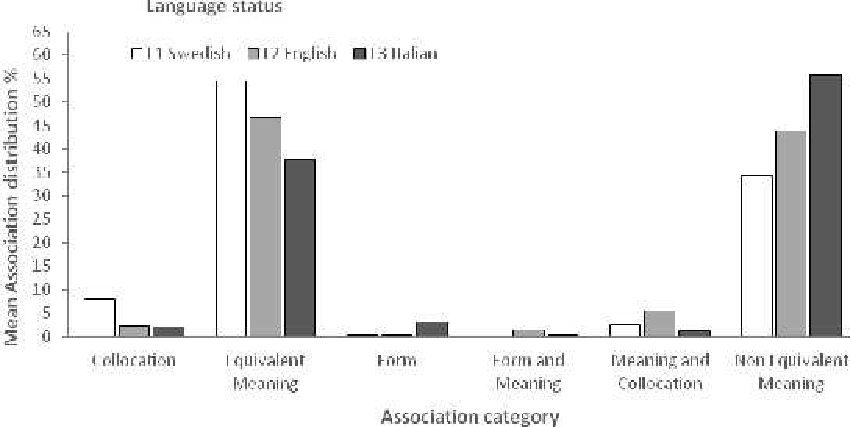
\includegraphics[width=\textwidth]{figures/Gudmundson-fig2.pdf}
    \caption{Association distribution in L1 Swedish, L2 English and L3 Italian and in the six association categories.}
    \label{fig:gudmundson:2}
\end{figure}

\begin{sidewaystable}
    \begin{tabular}{l *{3}{S[table-format=2.2] S[table-format=3.0] S[table-format=-1.2]} S[table-format=2.2] S[table-format=3.0] }
    \lsptoprule
         &  \multicolumn{3}{c}{Swedish} & \multicolumn{3}{c}{English} & \multicolumn{3}{c}{Italian} & \multicolumn{2}{c}{Tot.}\\\cmidrule(lr){2-4}\cmidrule(lr){5-7}\cmidrule(lr){8-10}\cmidrule(lr){11-12}
        Ass.    & {Ass.}       & {Obs.}    & {Stand.}      & {Ass.}       & {Obs.}     & {Stand.}      & {Ass.}       & {Obs.}   & {Stand.}      & {Ass.}       & {Obs.}\\
        cat. &  {dist.} &  {(\textit{N})} &  {res.} &  {dist.} & {(\textit{N})} &  {res.} & {dist.} &  {(\textit{N})} &   {res.} &  {dist.} &   {(\textit{N})}\\
    \midrule
        C  &  7.91 &  123 &    8.77 &  2.36 &   33 &  -4.40 &  2.06 &   26 &  -4.71 &  4.11 & 182\\
        EM & 54.60 &  849 &    7.63 & 46.67 &  652 &  -0.23 & 37.75 &  476 &  -7.80 & 46.34 & 1977\\
        F  &  0.06 &    1 &   -4.72 &  0.14 &    2 &  -3.99 &  3.17 &   40 &   9.08 &  1.13 & 43\\
        FM &  0.71 &   11 &   -0.43 &  1.43 &   20 &   3.36 &  0.16 &    2 &  -3.01 &  0.77 & 33\\
        MC &  2.38 &   37 &   -1.91 &  5.51 &   77 &   6.59 &  1.11 &   14 &  -4.77 &  3.00 & 128\\
        NM & 34.34 &  534 &   -9.57 & 43.88 &  613 &  -0.03 & 55.75 &  703 &  10.12 & 44.66 & 1850\\
        \midrule
        Tot. &     & 1555 &         &       & 1397 &         &       & 1261 &         & 16.67 & 4213\\
    \lspbottomrule
    \multicolumn{6}{l}{\parbox{6cm}{\footnotesize
    C = Collocational relation\\
    EM = Equivalent meaning relation\\
    F = Form-based relation\\
    FM = Form and meaning relation\\
    MC = Meaning and collocational relation    
    }} & \multicolumn{6}{l}{\parbox{6cm}{\footnotesize
    NM = Non-equivalent meaning relation\\
    Ass. cat. = Association category\\
    Ass. dist. = Association distribution\\
    Obs. = Observations\\
    Stand. res. = Standardized residuals}}
    \end{tabular}
    \caption{Association distribution, number of observations and standardized residuals for the different association categories and languages.\label{tab:gudmundson:2}}
\end{sidewaystable}

It can be noted that the greatest proportion of responses was of equivalent meaning or non-equivalent meaning type. These association categories stand out from the other categories in terms of number of associations. The third most common category was collocational, followed by the dual association category meaning and collocation. Form-based and form- and meaning-based associations were not that common. Form-based associations occurred almost only in the Italian data.

A first chi-square test of homogeneity showed that the association distribution was not homogeneously distributed over the different association categories, $\chi^2 (5, N = 4213) = 6302.3, p <0.000$. The second chi-square test of independence showed that the association distribution was not equally distributed over the different languages  $\chi^2(10, N = 4213) = 329.9, p <0.000$. As can be seen in \tabref{tab:gudmundson:3}, the association distribution in the Swedish data was significantly different from the one in the English data and from the Italian data, and the association distribution in the English data was significantly different from the one observed in the Italian data.

\begin{table}[p]
    \begin{tabular}{rcrrrl}
    \lsptoprule
         $\chi^2$ & df & \textit{n} & \textit{p}-value & Adj. alpha & Languages\\
    \midrule
        92.010 & 5 & 2952 & 0.000 & 0.010 & Swedish: English\\
        216.610 & 5 & 2816 & 0.000 & 0.010 & Swedish: Italian\\
        120.530 & 5 & 2658 & 0.000 & 0.010 & English: Italian\\
    \lspbottomrule
    \end{tabular}
    \caption{Pairwise comparisons between the three languages}
    \label{tab:gudmundson:3}
\end{table}

To follow up the chi-square test of independence, standardized residuals were analyzed. According to \citet[81]{Agresti2013}, “[a] standardized residual that exceeds about 2 or 3 in absolute value indicates lack of fit of $H_0$ in that cell”. The standardized residuals in the six categories and the three languages are visualized in \figref{fig:gudmundson:3}.

\begin{figure}[p]
\pgfplotstableread{
  %absolute
%   swe             eng         ita
1  8.76653472     -4.40236275  -4.71182177
2  7.63199404     -0.23336220  -7.80211753
3 -4.72373720     -3.99123434   9.08055903
4 -0.42740446      3.36227379  -3.00609634
5 -1.90556340      6.58865575  -4.76528859
6 -9.57433020     -0.02944098   10.11896941
}\dataset
\begin{tikzpicture}
\begin{axis}[%
        colormap/RdYlBu,
        cycle list name = langsci,
        line width=.75pt,
        sharp plot,
        width=.95\textwidth,
        ylabel={Standardized residuals},
        xlabel={Association category},
        xlabel style = {yshift=-8mm},
        xtick=data,
        xticklabels = {
            Collocation,
            Equivalent meaning,
            Form,
            Form and meaning,
            Meaning and collocation,
            Non-equivalent meaning
        },
        axis lines*=left,
        legend style={font=\footnotesize,at={(0.7,0.2)}},
        legend cell align=left,
        x tick label style={align=center,text width=2cm},
        ticklabel style = {font=\footnotesize},
        ]
\addplot  table[x index=0,y index=1] \dataset; %ano de 2013-2014
\addplot  table[x index=0,y index=2] \dataset; %ano de 2012-2013
\addplot  table[x index=0,y index=3] \dataset; %ano de 2011-2012
\legend{L1 Swedish,L2 English,L3 Italian}
\end{axis}
\end{tikzpicture}
%     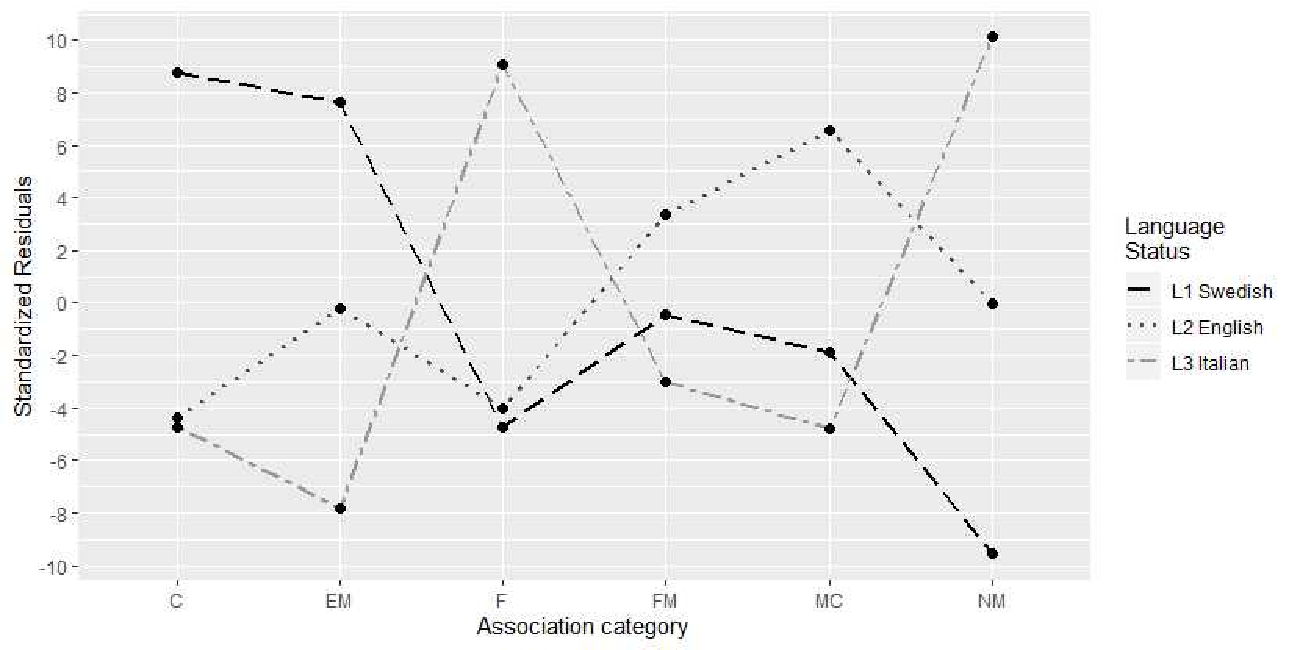
\includegraphics[width=\textwidth]{figures/Gudmundson-fig3.pdf}
%     \parbox{.5\textwidth}{
%     \footnotesize
%     C = Collocational relation\\
%     EM = Equivalent meaning relation\\
%     F = Form-based relation
%     }\parbox{.5\textwidth}{
%     \footnotesize
%     FM = Form and meaning relation\\
%     MC = Meaning and collocational relation\\
%     NM = Non-equivalent meaning relation\\
%     }
    \caption{Standardized residuals in the six association categories and the three languages: L1 Swedish, L2 English and L3 Italian.}
    \label{fig:gudmundson:3}
\end{figure}

The proportion of equivalent meaning associations in the Swedish data shows very large positive residuals, and we can infer that more L1 Swedish associations were of this type than if independence was true. The proportion of equivalent meaning associations in the L3 Italian data shows the opposite, i.e. very large negative values. The proportion of equivalent meaning associations in the L2 English data is exactly what is expected by the model. A large positive value is also found for collocational associations in L1 Swedish, while both L2 English and L3 Italian show large negative values. From \figref{fig:gudmundson:3} we can also infer that form-based associations are very common in L3 Italian, showing large positive values, while both L2 English and L1 Swedish show large negative values. The category non-equivalent meaning is associated with very large positive values in L3 Italian and with very large negative values in L1 Swedish. The same value for L2 English is not different from what had been expected if independence was true. The dual categories form and meaning relation and meaning and collocational relation indicate positive values for L2 English, while both L1 Swedish and L3 Italian show negative values. To sum up, three different aspects stand out. The first is that the L1 Swedish and L3 Italian data show the opposite behavior for values related to equivalent meaning associations and non-equivalent meaning association, but when it comes to the L2 English data, values for these two categories are the same and located just in between the data from L1 Swedish and L3 Italian. The second aspect is that collocational associations almost only occur in the L1 Swedish data, and the third aspect is that form-based associations almost only occur in the L3 Italian data.

\subsection{Reaction time: association categories and language status}\label{sec:gudmundson:3.2}

This section addresses research question 2, i.e. whether there is a difference in reaction times over the different association categories and, if so, if this difference could be related to language status. \tabref{tab:gudmundson:4} summarizes mean reaction times for the three languages and the six association categories, together with the number of observations and standard deviations. \figref{fig:gudmundson:4} illustrates mean reaction times in the three languages and the different categories.

\begin{table}
    \fittable{\begin{tabular}{l r r r r r r r r r r r r}
    \lsptoprule
        ~ &   \multicolumn{3}{c}{Swedish} & \multicolumn{3}{c}{English} & \multicolumn{3}{c}{Italian} & \multicolumn{3}{c}{Tot.}\\\cmidrule(lr){2-4}\cmidrule(lr){5-7}\cmidrule(lr){8-10}\cmidrule(lr){11-13}
        Ass.      & Obs.      & \textit{M}    &   & Obs.      & \textit{M}    &    & Obs.   & \textit{M}    &   & Obs.    & \textit{M}    &  \\
             cat. &      (\textit{N}) &            RT & SD &       (\textit{N})  &            RT & SD &      (\textit{N}) &            RT & SD &      (\textit{N}) &            RT & SD\\
    \midrule
        C    & 123 & 1966 & 808  &            {33}  & 1994 & 794  &        26  & 2761 & 1317 &           182 & 2084 & 932 \\
        EM   & 849 & 2169 & 1010 &            {652} & 2310 & 1012 &        476 & 2757 & 1246 &           1977& 2357 & 1097\\
        F    & 1   & 1537 &      &            {2}   & 1746 & 185  &         40 & 3315 & 1392 &           43  & 3201 & 1407\\
        FM   & 11  & 2641 & 969  &            {20}  & 2037 & 841  &        2   & 2967 & 1909 &           33  & 2295 & 969 \\
        MC   & 37  & 1914 & 799  &            {77}  & 1613 & 701  &        14  & 1627 & 510  &           128 & 1701 & 721 \\
        NM   & 534 & 2261 & 1114 &            {613} & 2550 & 1133 &        703 & 3184 & 1312 &           1850& 2707 & 1260\\
        Tot. & 1555& 2181 & 1032 &            {1397}& 2365 & 1070 &        1261& 3000 & 1308 &           4213& 2487 & 1184\\
    \lspbottomrule
    \multicolumn{7}{l}{%
    \parbox{6cm}{\footnotesize
    C = Collocational relation\\
    EM = Equivalent meaning relation\\
    F = Form-based relation\\
    FM = Form and meaning relation}}
    & \multicolumn{6}{l}{%
    \parbox{6cm}{\footnotesize
    MC = Meaning and collocational relation\\
    NM = Non-equivalent meaning relation\\
    RT = Reaction time\\
    \\}}
    \end{tabular}}
    \caption{Mean reaction times and number of observations for the different association categories and languages.\label{tab:gudmundson:4}}
\end{table}

When looking at the total values for the different languages, reaction times were fastest in Swedish, followed by English, followed by Italian. As regards the different categories, reaction times were fastest for meaning and collocational associations, i.e. a dual link between the cue word and the association implied fast responses. As far as that category is concerned, there were very small differences in response times across languages. The second fastest response times were obtained in collocational associations followed by equivalent meaning associations, i.e. associations with a significant semantic overlap. Form-based associations produced the slowest responses, even though response times for Swedish and English were rather fast. It is important, though, to recognize that the English and Swedish data are built on three observations only, and that the data, in general, are rather unbalanced.

\begin{figure}
\pgfplotstableread{
  %absolute
1  1966   1994  2084
2  2169   2310  2357
3  1537   1746  3201
4  2641   2037  2295
5  1914   1613  1701
6  2261   2550  2707

% relative
% 1
% 2
% 3
% 4
% 5
% 6
}\dataset
\begin{tikzpicture}
\begin{axis}[ybar,
        width=.95\textwidth,
        height=.3\textheight,
        ymin=0,
        ylabel={Mean association time},
        xlabel={Association category},
        xlabel style = {yshift=-8mm},
        xtick=data,
        bar width=4mm,
        xticklabels = {
            Collocation,
            Equivalent meaning,
            Form,
            Form and meaning,
            Meaning and collocation,
            Non-equivalent meaning
        },
        nodes near coords style={
            anchor=west,
            rotate=90,
            font = \footnotesize
            },
        axis y line*=left,
        axis x line*=bottom,
        legend style={font=\footnotesize},
        legend pos=south west,
        legend columns=-1,
        legend cell align=left,
        x tick label style={align=center,text width=2cm},
        ticklabel style = {font=\footnotesize},
        ]
\addplot[draw=black,fill=lsLightBlue, nodes near coords] table[x index=0,y index=1] \dataset; %ano de 2013-2014
\addplot[draw=black,fill=lsMidDarkBlue, nodes near coords] table[x index=0,y index=2] \dataset; %ano de 2012-2013
\addplot[draw=black,fill=lsNightBlue, nodes near coords] table[x index=0,y index=3] \dataset; %ano de 2011-2012
\legend{L1 Swedish,L2 English,L3 Italian}
\end{axis}
\end{tikzpicture}

%     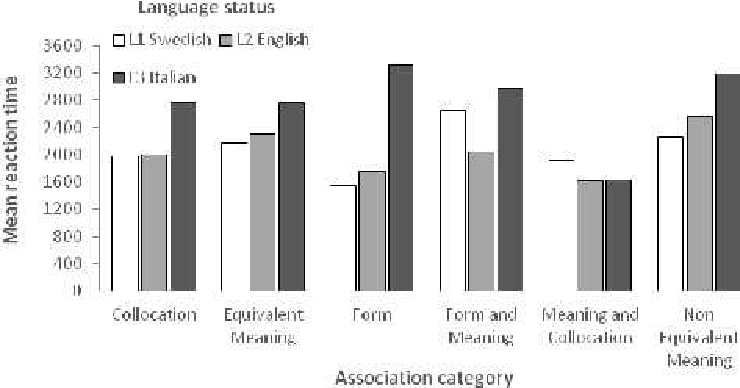
\includegraphics[width=\textwidth]{figures/Gudmundson-fig4.pdf}
    \caption{Word association task, mean reaction times over the different association categories and languages.}
    \label{fig:gudmundson:4}
\end{figure}

To verify whether language status and association category are associated with reaction time, a standard general linear model approach, assuming independent samples, was used. Since the distribution of the response time was skewed, a log transformation on the response time was applied, which resulted in an approximately normal distribution.

A significant effect ($F(2, 4210) = 201.8, p < 0.000$) of language status on reaction time was observed, and a significant effect of association category on reaction times $F(5, 4205) = 26.16, p < 0.000$. There was also a significant interaction effect between language status and association category $F(10, 4195) = 3.50, p < 0.000$. Following statistical reporting guidelines \citep{FieldEtAl2012}, pairwise comparisons were conducted on the significant interaction effect only. The comparisons are reported in \tabref{tab:gudmundson:5}. Only significant contrasts ($p \leq 0.05$) are reported. The last column reports effect size in terms of Cohen’s \textit{d}. \citet{Cohen1988} defined a small, a medium and a large effect size as corresponding to 0.2, 0.5 and 0.8, respectively.

\begin{table}
\small
    \begin{tabular}{>{\raggedright}p{3.85cm} S[table-format=-1.4] S[table-format=1.4] S[table-format=3.0] S[table-format=-1.4] S[table-format=<1.4] S[table-format=-1.2] }
    \lsptoprule
         Contrast & {Estimate} & {\textit{SE}} & {df} & {\textit{t}-ratio} & {\textit{p}-value\footnote{Comparisons were made with the Tukey’s HSD method}} & {\textit{d}}\\
    \midrule
      Equivalent meaning & & \\
        Swedish -- English & -0.0712 & 0.0220 & 4195 & -3.229 & 0.0036 & -0.17\\
        Swedish -- Italian & -0.0254 & 0.0914 & 4195 & -9.780 & <0.0001 & -0.56\\
        English -- Italian & -0.1659 & 0.0255 & 4195 & -6.500 & <0.0001 & -0.39\\
        \tablevspace
        Collocation & & \\
        Swedish -- Italian & -0.3041 & 0.0914 & 4195 & -3.328 & 0.0025 & -0.72\\
        English -- Italian & -0.2787 & 0.1110 & 4195 & -2.511 & 0.0324 & -0.66\\
        \tablevspace
        Non-equivalent meaning & & \\
        Swedish -- English & -0.1361 & 0.0251 & 4195 & -5.432 & <0.0001 & -0.32\\
        Swedish -- Italian & -0.3618 & 0.0243 & 4195 & -14.888 & <0.0001 & -0.85\\
        English -- Italian & -0.2257 & 0.0234 & 4195 & -9.647 & <0.0001 & -0.53\\
        \tablevspace
        English & & \\
        Equivalent meaning -- Meaning and collocation & 0.34828 & 0.0510 & 4195 & 6.828 & <0.0001 & 0,42\\
        Equivalent meaning -- Non-equivalent meaning & -0.09543 & 0.0238 & 4195 & -4.007 & 0.0009 & -0.23\\
        Collocation -- Non-equivalent meaning & -0.22219 & 0.0756 & 4195 & -2.937 & 0.0390 & -0.52\\
        Meaning and collocation -- Non-equivalent meaning & -0.44372 & 0.0512 & 4195 & -8.670 & <0.0001 & -1.05\\
        \tablevspace
        Italian & & \\
        Equivalent meaning -- Form & -0.18901 & 0.0697 & 4195 & -2.712 & 0.0730 & -0.45\\
        Equivalent meaning -- Meaning and collocation & 0.47666 & 0.1148 & 4195 & 4.153 & 0.0005 & 1.13\\
        Equivalent meaning -- Non-equivalent meaning & -0.15520 & 0.0251 & 4195 & -6.177 & <0.0001 & -0.37\\
        Collocation -- Meaning and collocation & 0.46274 & 0.1403 & 4195 & 3.298 & 0.0126 & 1.09\\
        Form -- Meaning and collocation & 0.66567 & 0.1315 & 4195 & 5.064 & <0.0001 & 1.57\\
        Meaning and collocation -- Non-equivalent meaning & -0.63187 & 0.1143 & 4195 & -5.530 & <0.0001 & -1.49\\
    \lspbottomrule
    \end{tabular}
    \caption{Interaction effects: pairwise comparisons of RT\label{tab:gudmundson:5}}
\end{table}

If we start by looking at the two largest association categories – equivalent meaning and non-equivalent meaning – there are significant differences between all languages. These associations are produced faster in Swedish compared to English and faster in English compared to Italian. In terms of effect size, for the equivalent meaning associations, the difference between Swedish and English, and English and Italian, could be considered small, while the difference between Swedish and Italian is of medium size. When looking at the non-equivalent meaning associations, there is a small effect between Swedish and English, a medium effect between English and Italian and a large effect between Swedish and Italian. Collocational associations are significantly faster in Swedish than in Italian, and also significantly faster in English than in Italian, and those effects are rather large. No other significant differences between the three languages could be observed. It must be recognized, though, that the number of responses in the other categories is not large enough to produce reliable data. If we look at differences in reaction times between the categories within the three languages, results show there are no significant differences in Swedish. For English, on the other hand, there are significant differences between equivalent meaning and meaning and collocational associations, between equivalent meaning and non-equivalent meaning associations, between collocational and non-equivalent meaning associations and, finally, between meaning and collocational associations and non-equivalent meaning associations. Among these, the last comparison is associated with a large effect size, while the other three are associated with medium or small effect sizes. The Italian data reveal large differences in reaction times between many different categories. Significant differences in reaction times are observed between the categories equivalent meaning and form, equivalent meaning and meaning and collocation, equivalent meaning and non-equivalent meaning, collocation and meaning and collocation and, finally, meaning and collocation and non-equivalent meaning. A difference between equivalent meaning associations and form-based associations that approached a \textit{p-}value of 0.05 (0.07) was also detected.  The effect sizes in Italian are generally very large. To sum up, reaction times for the two largest categories, equivalent meaning and non-equivalent meaning, are fastest in L1 Swedish, followed by L2 English, followed by L3 Italian. As concerns the third largest category, collocations, no difference was observed between Swedish and English. The number of significant differences observed between the different categories within each language was six in L3 Italian, four in L2 English and none in L1 Swedish. The effect sizes in the Italian data were also much larger compared to the English data.

\subsection{Long-term cross-language semantic priming}\label{sec:gudmundson:3.3}

This section refers to research question 3, i.e. whether it is possible to obtain a long-term cross-language semantic priming effect between L3 and L2, and if semantic activation of an L3 word co-activates, or requires mediation of, the corresponding L2 word. Results from the LDT are listed in \tabref{tab:gudmundson:6}. \tabref{tab:gudmundson:6} reports mean reaction times and standard deviations for the two conditions of translation equivalent (primed condition) and control word (non-primed condition). Participants responded faster (629.77) to the primed items than to the control words (656.22). A mean difference of 26.45 milliseconds was observed between the primed and the non-primed condition.

\begin{table}
\small
    \begin{tabularx}{\textwidth}{lR{3.5cm}R{2.5cm}R{4.5cm}c}
    \lsptoprule
        ~ & Translation equivalent (primed) & Control word\newline\noindent(non primed) & Difference between primed and non-primed condition\\
    \midrule
        \textit{M} & 629.77 & 656.22 & 26.45\\
        SD & 101.43 & 110.50 & \\
    \lspbottomrule
    \end{tabularx}
    \caption{Mean reaction times for non-words, primed words and non-primed words}
    \label{tab:gudmundson:6}
\end{table}

A \textit{t}-test indicated a significant effect of priming on reaction times, $t(18) = 4.23, p < 0.000$, two-tailed. Reaction times for control words were significantly slower than reaction times for translation equivalents.

\section{Discussion}\label{sec:gudmundson:4}

The discussion section includes two subsections. In the first, a discussion related to the word association tasks is presented. This subsection considers both the association distribution data and the reaction time data, i.e. research questions 1 and 2. That is because a combined analysis of these two research questions is believed to be more fruitful and meaningful when it comes to understanding how the multilingual lexicon grows and evolves. \sectref{sec:gudmundson:4.2} discusses research question 3, i.e. results from the LDT and the long-term cross-language semantic priming effect observed between L3 Italian and L2 English.

\subsection{Association distribution and response times in word association}\label{sec:gudmundson:4.1}

Generally, the word association data showed that participants in the study preferred equivalent meaning and non-equivalent meaning associations in all languages, and that other kinds of responses occurred rarely. However, differences between the languages were found and it could be concluded that the association distribution differed according to language status and association category. Form-based associations occurred almost only in the L3 (Italian), whereas the proportion of collocational associations in the L1 (Swedish) was very high compared to both the L2 (English) and L3 (Italian). The last two showed similar values. In L1 Swedish, the most common association category was of equivalent meaning, while in L3 Italian, the most common association category was of non-equivalent meaning. As regards L2 English, associations expressed equivalent and non-equivalent meaning to the same extent. In other words, the proportion of equivalent meaning associations increased from the L3 to the L2 and from the L2 to the L1. On the other hand, the proportion of non-equivalent meaning associations showed the opposite behavior, i.e. they increased from the L1 to the L2 and from the L2 to the L3. Thus, the proportion of equivalent meaning versus non-equivalent meaning associations varies according to language status, a trend that resembles the traditional syntagmatic-paradigmatic shift observed in other word association studies within L1 and L2 research (\citealt{Ervin1961, EntwisleEtAl1964, Meara1978, Politzer1978, FitzpatrickIzura2011, KhazaeenezhadAlibabaee2013}).

As regards reaction times, results showed that these changed with language status, hence, fastest reaction times were obtained in L1 Swedish, followed by L2 English, and finally L3 Italian. This is what would be predicted by the RHM, i.e. longer response latencies when associating in a weaker second language since the only way to access semantic information is through the L1. Additionally, with increasing proficiency, learners should be less dependent on L1 conceptual mediation. Another possible, and simpler, explanation of the reaction time differences between the languages is fluency or automaticity, i.e. lexical access is more fluent in the L1 than in the L2, and more fluent in the L2 than in the L3.\largerpage

Results showed an interaction effect between language status and association category on reaction time. As regards the largest categories, equivalent meaning and non-equivalent meaning, differences in reaction times between all languages were observed; association times were faster in L1 Swedish followed by L2 English and, finally, L3 Italian. When it comes to collocations on the other hand, even if differences in reaction times were found between Swedish and Italian, and Italian and English, no difference could be observed between Swedish and English, even if collocational associations were much more common in Swedish compared to English. An interesting fact is that there were no statistical differences in reaction times between the association categories in the Swedish data, while differences were observed both in English and in Italian. It should also be observed that more differences were found in the Italian data compared to the English data. These results indicate a trend according to which reaction times in the different categories are evened out with language status or with increasing proficiency and fluency. When a language user has reached a high level of proficiency, lexical retrieval is fast in all categories. A difference in reaction times between different association categories is most easily detected in less proficient language users.

As already mentioned, form-based associations occurred almost only in the L3 (Italian): while participants produced, in total, one form-based association in the L1 Swedish and two form-based associations in the L2 English, they produced as many as 40 form-based associations in the L3. Among these, we find \textit{aquila} – \textit{acqua} (‘eagle’ -- ’water’), \textit{cuscino} – \textit{cucina} (‘pillow’ – ‘kitchen’), and \textit{doccia} – \textit{dolce} (‘shower’ – ‘cake’), i.e. words that have no obvious conceptual overlap, but are related only by phonological or orthographic characteristics and word class. It is known that words that share orthographic and phonological features co-activate (\citealt{VanHeuvenEtAl1998, Aitchison2012}), and earlier studies have shown that these associations are particularly common in the L2 (\citealt{Meara1978, FitzpatrickIzura2011}) and that they diminish with increasing proficiency (\citealt{RiegelZivian1972}). The large proportion of form-based associations in Italian might be due to the fact that only form-based links existed between the cue word and other words in the mental lexicon, simply because the meaning of the word was unknown and therefore failed in activating words with related meaning. Another possibility would be that the word was not unknown and that conceptual links to other words did exist, but that they were less strong compared to the orthographic links due to a limited vocabulary. \citeauthor{EllisN1996} states, “[a]t the point in acquisition when a particular representation is salient, that representation has a higher likelihood of driving word association responses” (\citeyear[93]{EllisN1996}). As proposed by \citet{Nation2001}, and \citet{HaastrupHenriksen2000}, depth (i.e., a word’s different sense relations) increases with breadth, which means that it is not until a learner has a large enough vocabulary that she or he can start to make use of conceptual links between words. This also gives support to the RHM that claims that the connections between forms and concepts are weak in languages where proficiency is low (\citealt{KrollStewart1994}). As regards reaction times, form-based associations in Italian were slower compared to the other association categories. This could be explained, either by the fact that phonological or orthographic links were less strong compared to semantically related links, or by the fact that participants started out by looking for a semantically related word, failed and instead chose an orthographically or phonologically similar word. The latter explanation implies that semantic, as well as and orthographic and phonological links could be equally strong, but that participants performed additional steps when making a form-based association.

Collocations were mainly produced in L1 Swedish,\largerpage
and rarely in L2 English or in L3 Italian. It thus seems that the use of collocational links is something that characterizes L1 behavior and makes it different from other languages learned. \citet{Fitzpatrick2006} found that collocational responses were more common in native speakers compared to non-native speakers and that no correlation as concerns the proportion of collocations between learners at different proficiency levels was revealed. This result was replicated in the present study in the sense that participants produced significantly more collocational responses in L1 Swedish compared to both L2 English and L3 Italian. No difference was found between L2 English and L3 Italian, despite the fact that proficiency was generally higher in L2 English. These results are consistent with chunking theories (e.g. \citealt{EllisN1996, Wray2002}) that consider language, due to processing advantages, to be stored in chunks. These chunks are processed faster as a result of frequency of practice. According to \citet[110]{Sinclair1991}, “[a] language user has available to him or her a large number of semi-preconstructed phrases”, but \citet{Wray2002} claims that this is true for native speakers only; native speakers store language in bigger chunks, while non-native speakers retrieve them word by word. This has also been confirmed by research on advanced L2 speakers that show that collocations are learned late during the acquisition phase (for an overview see \citealt{ErmanEtAl2016}). As far as reaction times are concerned, according to \citet[141]{ErmanEtAl2016}, formulaic sequences are processed more quickly than non-formulaic sequences and, even though processing times are generally slower for non-native speakers, this observation holds true for both native and non-native speakers. The present study confirmed this; collocational associations obtained the second fastest response times. It is interesting to notice that no differences in reaction times for collocational associations were observed between English and Swedish, i.e. even if collocational associations were much more common in the Swedish data, when they appeared in English, reaction times were not different from the ones obtained in Swedish. Fastest reaction times in total were obtained when the association category was of the dual-link response type meaning and collocation. Among the associations belonging to the dual-link category meaning and collocation we find \textit{uovo} -- \textit{gallina} (‘egg’ -- ‘hen’), \textit{uomo} -- \textit{donna} (‘man’ -- ‘woman’), \textit{dawn} -- \textit{dusk, nail} -- \textit{finger, body-soul, korv-bröd} (‘hot dog’ -- ‘bread’), \textit{nyckel – dörr} (‘key’ -- ‘door’) \textit{tröja-polo} (‘sweater’ -- ‘polo’). These words are connected to each other both by the fact that they often co-occur syntagmatically in language, but also by the fact that they share some kind of equivalent meaning such as hyperonymy, iperonymy or partonymy. They are, so to say, well-rehearsed and connected by strong semantic links. The fact that reaction times were similar in all languages implies that fluency for some lexical connections in additional languages can be at the same level as those of native speakers.

\citet{CremerEtAl2010} pointed out that it was still uncertain to what extent L1 or L2 speakers act as homogeneous groups and how their word association responses distribute over different response categories. \citeauthor{CremerEtAl2010} also observed that even less is known about word association patterns in multilinguals. Overall, in the present study, results in the three languages were similar in nature, and the observed differences could be attributed to quantitative or developmental differences rather than to qualitative differences related to processing mechanisms or representation. Reaction times increase in the following order, if form-based relations and form and meaning relations are excluded: meaning and collocation, collocation, equivalent meaning and non-equivalent meaning. The fact that associations generally were produced faster in L1 Swedish, followed by L2 English and L3 Italian, respectively should be attributed to differences in fluency, or proficiency, and not to differences in processing itself. Other differences in association behavior that could be attributed to developmental changes or proficiency were the shift from non-equivalent meaning associations to equivalent meaning associations with language status, the high proportion of form-based associations in L3 Italian compared to the other two languages, and the high proportion of collocational associations in L1 Swedish compared to the two non-native languages. The results suggest a developmental trend that is similar, but not identical, to the one discussed by \citet[94]{EllisN1996} who states that in the mental lexicon: “both [in] the L1 and L2, lexical items are first represented as ordered phonological strings then there is a focus on their collocations and their sequential probabilities in word strings, and only later are these patterns of occurrence analyzed to allow syntactic and semantic classification.”

Results from the present study actually suggest a slightly different progression, where semantic classification precedes the focus on sequential probabilities, i.e. learners seem to be able to create strong semantic networks without being able to handle collocations and collocational probabilities, even if they are produced fast when they do occur. \citet{DallerEtAl2007} propose a three-dimensional model to illustrate word knowledge. The three dimensions – breadth, fluency and depth~– constitute a so-called lexical space in which the lexical knowledge of a learner can be located. They argue that some learners might, for example, show a high degree of fluency, but poor lexical breadth, or large vocabularies, but poor fluency. In what follows, a model of the developing mental lexicon composed of four different dimensions – vocabulary breadth and depth, fluency, proficiency and association category – is proposed, but it must be understood as hypothetical (\figref{fig:gudmundson:5}).

\begin{figure}
    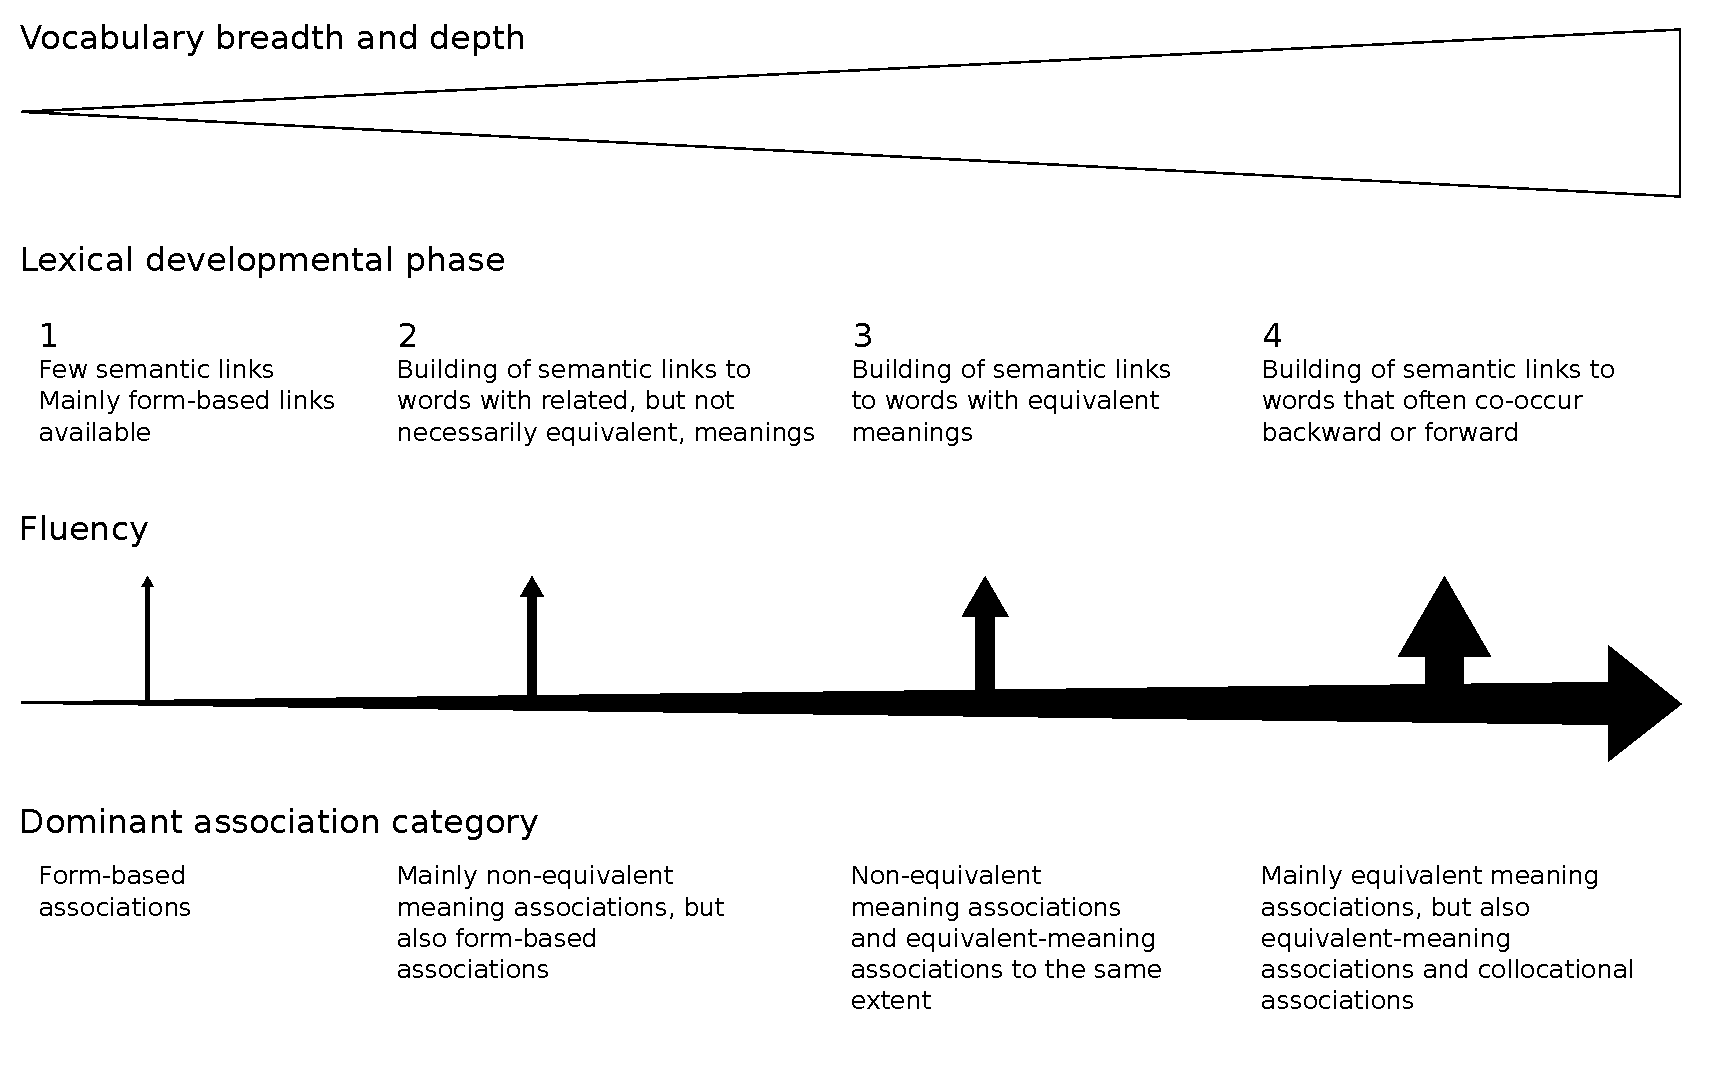
\includegraphics[width=\textwidth]{figures/Gudmundson-fig5mod.pdf}
    \caption{Model of the developing mental lexicon.}
    \label{fig:gudmundson:5}
\end{figure}

The model proposed in \figref{fig:gudmundson:5} suggests that the connections in the mental lexicon grow in four steps in relation to increasing vocabulary breadth and depth. As discussed in \sectref{sec:gudmundson:1.1}, these two categories are interdependent and develop in parallel – growing breadth also leads to growing depth. These steps are not to be viewed as discrete phases but rather as a continuum. The learner starts from building form-based links in the first phase since no or few semantic links are available when a word is unknown. In this step, mostly form-based associations can be performed (\textit{book-hook}). In the second step, due to increasing vocabulary breadth and depth, the learner starts to create semantic relations between words with related meanings or to words that appear in the same semantic context (\textit{book-glasses}). Due to a limited vocabulary, few links to words with equivalent meanings, such as synonyms, are available, and therefore associations are mostly of non-equivalent meaning. In the third phase, the number of words known by a learner has increased enough to include connections between words with equivalent meanings and the learner can start to produce associations based on synonymy or partonymy (\textit{book-volume} or \textit{book-pages}). In the last phase, learners start to build collocational links to words that normally co-occur backward or forward and the amount of collocational word associations increases (\textit{book-title}). Fluency works in two different dimensions. The first dimension is related to language proficiency and is represented by the horizontal arrow. It presupposes that learners get more fluent and automatic in their word retrieval as they get more proficient. The second dimension of fluency is related to the different kinds of association categories or lexical links in the mental lexicon, and is represented by vertical arrows. Some associations, such as the one of equivalent meaning type, are produced faster due to large semantic overlap or frequent co-occurrence, and therefore represented with thicker arrows. The distinction between two different fluency dimensions might explain why some associations are faster than others within a language, but also differences between languages and as such differences related to proficiency. A collocational association such as \textit{book-title}, if produced by a low proficiency language learner with poor fluency, might be faster than a non-equivalent meaning association such as \textit{book-glasses}, if produced by a more proficient language learner of the same language or even by a native speaker. Speed of association, and therefore fluency, is not only a question of proficiency but also a question of association category. According to the model in \figref{fig:gudmundson:5}, the lexical development of the various languages known by a learner might have reached different phases. In the present study, for example, the L1 could be said to have reached phase, 4 while the L2 could be said to have reached phase 3. The L3, on the other hand, seems to have reached only phase 2.

\subsection{Long-term semantic priming and lexical mediation between the L3 and the L2}\label{sec:gudmundson:4.2}\largerpage

The LDT reported in this study proved that during L3 production that required semantic activation (the word association task in L3), the corresponding L2 translation equivalent was unconsciously activated. Most likely, the L1 translation equivalent was also activated, but this effect is not controlled for in this study. This research is in line with results in the bilingual domain and can now be extended to a multilingual context and to a new language combination. Both \citet{FitzpatrickIzura2011} and \citet{LiEtAl2009} found an effect of long-term cross-language semantic priming between L2 and L1 that indicated that during L2 conceptual processing, the corresponding L1 translation equivalent had also been activated. Both interpreted the results in favor of the RHM, i.e. that L1 has a special status in acting as conceptual mediator in low proficient L2 users. The mediating effect of the L1 during the word association task postulated by \citet{FitzpatrickIzura2011} was depicted in the way presented in \figref{fig:gudmundson:6}.

\begin{figure}
\fbox{\parbox{.8\textwidth}{
\centering
~\hfill Intermediate L1 link \hfill~\\
Cue word (L2) \hfill Response (L2)\\
 \hfill \textbf{LORRY} \hfill \tikzfancyarrow{}  \hfill\textit{camión} `lorry' \hfill \tikzfancyarrow{}  \hfill \textbf{CAR} \hfill~\\
 }}
%     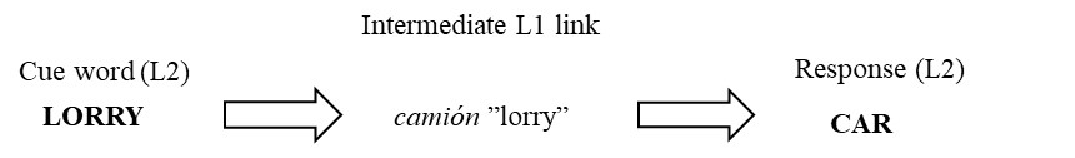
\includegraphics[width=\textwidth]{figures/Gudmundson-fig6.pdf}
    \caption{Mediation effect of the L1 Spanish during the L2 English word association task. Adapted from \citet{FitzpatrickIzura2011}.}
    \label{fig:gudmundson:6}
\end{figure}

In the present study, a priming effect of 26.45 milliseconds was observed between L3 and L2 in the LDT, which was similar to the one obtained by Fitzpatrick \& Izura of 20 milliseconds between L2 and L1. If we assume that conceptual access proceeds in the way postulated by the RHM (i.e., that L1 mediates conceptual access in a later learned language), it needs to be added to the model that also another non-native language could fill the same function. Such a model would look like the one presented below in \figref{fig:gudmundson:7}.

\begin{figure}
\fbox{\parbox{25mm}{\centering
Cue word (L3)\\\smallskip

\textbf{TAVOLA}\\
`table'\medskip\\~
}
\parbox{15mm}{
\rotatebox[origin=c]{20}{\tikzfancyarrow[1.5cm]}\\
\rotatebox[origin=c]{-20}{\tikzfancyarrow[1.5cm]}\\
}
\parbox{35mm}{\centering
Intermediate L1 link\\\smallskip
\textit{bord} `table'\\\bigskip
Intermediate L2 link\\\smallskip
\textit{table}
}
\parbox{15mm}{
\rotatebox[origin=c]{-20}{\tikzfancyarrow[1.5cm]}\\
\rotatebox[origin=c]{20}{\tikzfancyarrow[1.5cm]}\\
}
\parbox{25mm}{\centering
Response (L3)\\\smallskip
\textbf{SEDIA}\\
`chair'\medskip\\~
}}
%     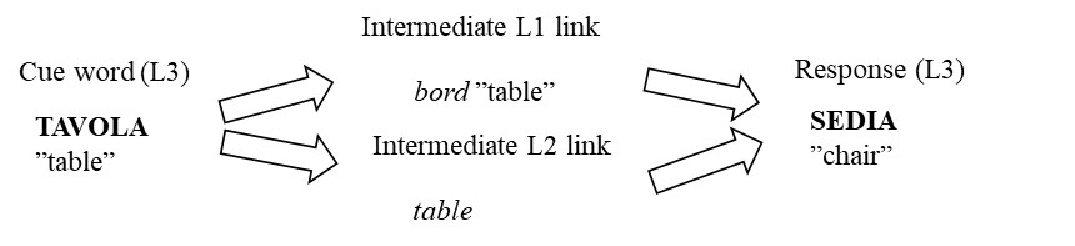
\includegraphics[width=\textwidth]{figures/Gudmundson-fig7.pdf}
    \caption{Mediation effect of the L2 and the L1 during the L3 word association task.}
    \label{fig:gudmundson:7}
\end{figure}

\citet{Abunuwara1992} favored a model where all non-native languages relate and depend on L1 only, but the present results could be said to imply that L1 is not unique or qualitatively different from an L2 when it comes to mediating semantic access. As stated by \citeauthor{Szubko-Sitarek2011}, “it seems legitimate to say that the native language does not always have a privileged status” (\citeyear[170]{Szubko-Sitarek2011}).

Generally, in studies of multilingual lexical processing, the L3 is the weakest language, which makes it difficult to distinguish between language status and proficiency, and this is the case in the present study. We cannot know whether the results are due to the fact that English was learned before Italian or due to the fact that proficiency was higher in English. \citeauthor{GoralEtAl2006} suggest that “a third language (L3) may be learned in connection with a previously learned non-native language (L2), and thus develop strong lexical connections with that language” (\citeyear[244]{GoralEtAl2006}), and that might be independent of proficiency. It can also be added that we do not know anything about the size of the different arrows in \figref{fig:gudmundson:7}. It might be, for example, that the effect is stronger in the L1 compared to the L2, but it must be noted that that the priming effect, expressed in milliseconds, was slightly higher in this study compared to the study by \citet{FitzpatrickIzura2011}.

It is difficult to understand how the RHM would account for multilingualism and how to adapt it to a situation with more than one non-native language. How would the relation between the non-native languages be represented, and when translating between two non-native languages, what would be considered backward and forward translation respectively? Few studies treat the relation between L2 and L3, and more research is needed to understand how and what kind of connections develop between an L3 and a speaker’s L1 and L2 respectively from a coordinate or subordinate approach. Results in the present study are more easily explained by a model such as the BIA+ that presupposes activation spreading and co-activation of all known languages. The non-selective access approach is also supported by studies on the cognate effect in trilinguals (\citealt{LemhöferEtAl2004, Szubko-Sitarek2011}). A general problem with the BIA+ model is that it does not take into account proficiency, language status and typology, factors that all seem to play a crucial role in multilingual lexical access. A future model of multilingual language processing would benefit from incorporating these factors.

\section{Conclusion}\label{sec:gudmundson:5}

Results in the present study of the mental lexicon of multilingual speakers point in the direction that lexical representations, access and development proceed similarly in all languages known by a trilingual language user, and that the L1 is not qualitatively different from non-native languages. Differences in association behavior (i.e., the proportion of associations in the different categories) and the speed with which associations are produced are best explained by proficiency and fluency, i.e. by the fact that languages have reached different phases in their overall and lexical development. Results also favor non-selective access and co-activation of all languages during processing. A long-term semantic priming effect was found between L3 and L2 that proved that, during L3 lexical access, the L2 was activated. This does not exclude the possibility that the corresponding L1 semantic and lexical representations were also active.

Future studies would benefit from collecting data that can discriminate language status from proficiency, i.e. studying participants whose weakest language is the L2 and not the L3, but also data that can shed light on the role of both L1 and L2 when processing L3, or the role of L3 when processing L2 or L1. The present study has only investigated high frequency nouns and in the future, besides controlling for proficiency in L2 and L3, it would be useful to investigate other word types with various frequencies.

{\sloppy\printbibliography[heading=subbibliography,notkeyword=this]}
\end{document}
